\documentclass[xcolor=pdftex,dvipsnames,table,mathserif]{beamer}
\usepackage{subfigure}
\usepackage{amsbsy}
\usepackage{tikz}
\usetikzlibrary{arrows}
\usepackage{amsmath,graphicx,dsfont,color}
\usepackage{amsfonts}
\usepackage{amssymb}
\usepackage{array}

\bibliographystyle{apalike}

\setbeamertemplate{bibliography item}{\insertbiblabel}
\setbeamertemplate{bibliography entry title}{}
\setbeamertemplate{bibliography entry location}{}
\setbeamertemplate{bibliography entry note}{}

%Definitiona

\newcommand{\x}{\mathbf{x}}
\newcommand{\X}{\mathbf{X}}
\newcommand{\W}{\mathbf{W}} %Weight
\newcommand{\bais}{\mathbf{b}}%Bais
\newcommand{\act}{\texttt{g}}%Activation
\newcommand{\loss}{L}
\newcommand{\pdata}{\hat{p}_{\texttt{data}}}
\newcommand{\nsize}{n}
\newcommand{\param}{\boldsymbol{\theta}}
\newcommand{\featmap}{\boldsymbol{\phi}}
\newcommand{\EV}{\mathbb{E}}







\usepackage{physics}

\graphicspath{{../graphics/}}

\AtBeginSection[]{
  \begin{frame}{Contents}
    \tableofcontents[currentsection, hideothersubsections]
  \end{frame}
}

\AtBeginSubsection[]{
  \begin{frame}{Contents}
    \tableofcontents[currentsection, subsectionstyle=show/shaded/hide]
  \end{frame}
}

\setbeamertemplate{footline}[frame number]{}
\setbeamertemplate{navigation symbols}{}
\setbeamertemplate{section in toc}[square]
\setbeamertemplate{items}[square]

%% For image credits on image bottom right
\usepackage[absolute,overlay]{textpos}
\setbeamercolor{framesource}{fg=gray}
\setbeamerfont{framesource}{size=\tiny}
\newcommand{\source}[1]{\begin{textblock*}{4cm}(8.7cm,8.6cm)
    \begin{beamercolorbox}[ht=0.5cm,right]{framesource}
        \usebeamerfont{framesource}\usebeamercolor[fg]{framesource} Credits: {#1}
    \end{beamercolorbox}
\end{textblock*}}


\title{Practical recommendations}
\author{E. Decencière}
\date{MINES ParisTech\\
  PSL Research University\\
  Center for Mathematical Morphology
}
\titlegraphic{
\includegraphics[height=1.7cm]{../graphics/logoemp}}

\useinnertheme{rounded}
\usecolortheme{rose}

%%%%%%%%%%%%%%%%%%%%%%%%%%%%%%%%%%%%%%%%%%%%%%%%%%%%%%%
%%%%%%%%%%%%%%%%%%%%%%%%%%%%%%%%%%%%%%%%%%%%%%%%%%%%%%%

\begin{document}

\frame{\titlepage}

\frame{
  \frametitle{Contents}
  \tableofcontents[hidesubsections]
}

%%%%%%%%%%%%%%%%%%%%%%%%%%%%%%%%%%%%%%%%%%%%%%%%%%
%%%%%%%%%%%%%%%%%%%%%%%%%%%%%%%%%%%%%%%%%%%%%%%%%%
\section{Introduction}


%%%%%%%%%%%%%%%%%%%%%%%%%%%%%%%%%%%%
\begin{frame}{}
\centering
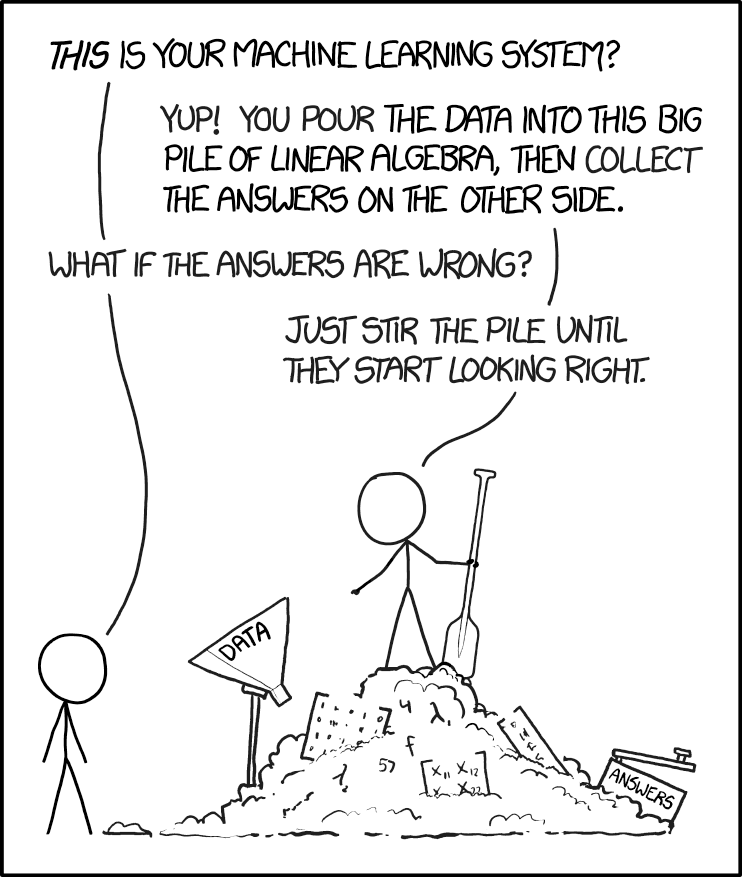
\includegraphics[height=\textheight]{xkcd_machine_learning}
\source{xkcd.com\\ (CC BY-NC 2.5)}
\end{frame}

%%%%%%%%%%%%%%%%%%%%%%%%%%%%%%%%%%%%
\begin{frame}{Practicing deep learning}

  In every discipline theory and practice are important. In deep learning, practice is essential.

  \begin{itemize}[<+->]
  \item We lack theoretical understanding of the success of deep learning
  \item Many common techniques have been adopted for empirical reasons
  \item In order to improve your skills, you have to practice a lot and read the reports by other practitioners
  \end{itemize}

  \pause

  \begin{alertblock}{}
    This state of affairs can of course be a problem in domains where security is important, such as clinical applications.
  \end{alertblock}

\end{frame}


%%%%%%%%%%%%%%%%%%%%%%%%%%%%%%%%%%%%%%%%%%%%%%%%%%%%%
\frame{
  \frametitle{General recommendations}

  \begin {itemize}[<+->]
  \item Familiarize yourself with the problem and the data
  \item Choose the right representation for your images
  \item Choose an architecture and train it
  \item Analyze the results on the validation data (\alert{look} at the images!)
  \item Beware of over-fitting! Envision regularization methods.
  \item Use data augmentation. If correctly used, it cannot hurt and will probably improve the generalization power of your network.
  \item Do you need preprocessing? Post-processing?
  \item Iterate, while precisely logging all your experiments.
  \item Only at the end: test!
  \end{itemize}
}



%%%%%%%%%%%%%%%%%%%%%%%%%%%%%%%%%%%%%%%%%%%%%%%%%%
\section{Problem representation}

%%%%%%%%%%%%%%%%%%%%%%%%%%%%%%%%%%%%%%%%%%%%%%%%%%%%%
\frame{
  \frametitle{Modeling your problem}

  Cast your problem into a convenient representation.

    \begin {itemize}[<+->]
    \item Understand the problem definition - discuss with the end-user
    \item Familiarize yourself with the data (input and output images)
    \item Choose the right representation for your images. Resolution? What labels?
    \end{itemize}


}


%%%%%%%%%%%%%%%%%%%%%%%%%%%%%%%%%%%%
\begin{frame}{Example: eye fundus image quality}

\begin{columns}
  \begin{column}{.4\textwidth}
    \begin{figure}[ht]
      \centering
      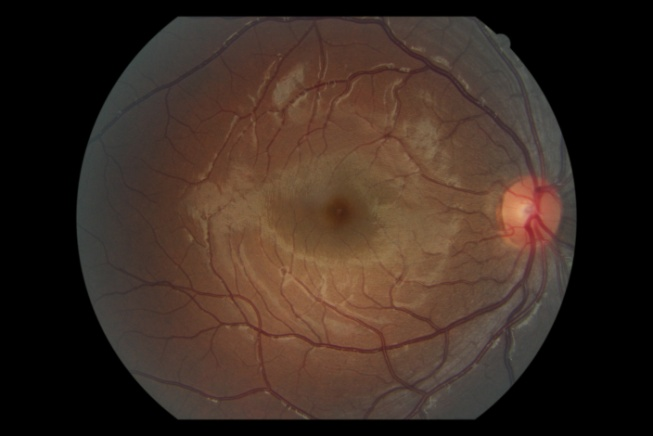
\includegraphics[width=\textwidth]{fundus1}\\
      Good quality\vspace{1em}\\
      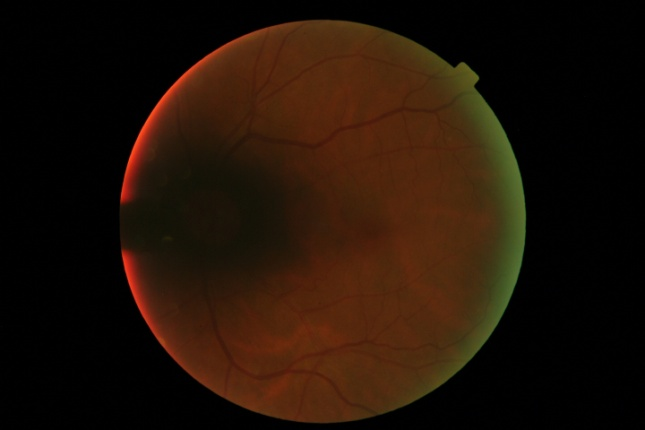
\includegraphics[width=\textwidth]{fundus2}\\
      Low quality
    \end{figure}

  \end{column}

  \begin{column}{.6\textwidth}
    \begin{itemize}[<+->]
    \item Quality criterion: are the macula and peripheral vessels visible?
    \item First solution: regression (center of macula position)
    \item Second solution: predict macula mask
    \end{itemize}
  \end{column}
\end{columns}

\source{images from OPHDIAT database}
\end{frame}

%%%%%%%%%%%%%%%%%%%%%%%%%%%%%%%%%%%%
\begin{frame}{Performance evaluation}

  \begin{itemize}
  \item Choose the right metrics and try to use a loss function that is as close as possible to these metrics
  \item Define an objective
  \end{itemize}

\end{frame}


%%%%%%%%%%%%%%%%%%%%%%%%%%%%%%%%%%%%%%%%%%%%%%%%%%%%%
\section{Data preparation}

%%%%%%%%%%%%%%%%%%%%%%%%%%%%%%%%%%%%
\begin{frame}{Building the data sets}
  \begin{itemize}
  \item Gather your images in order to build a data set that conveniently represents your problem
  \item How many images do you need?
  \item Build a proper ground-truth
  \end{itemize}

  \pause

  \begin{alertblock}{Is database constitution the main step?}
    \begin{itemize}
    \item In practical, real-world applications, this is becoming the most time-consuming step
    \item If the data set does not conveniently represent your problem you will run into difficulties
    \end{itemize}

  \end{alertblock}

\end{frame}

%%%%%%%%%%%%%%%%%%%%%%%%%%%%%%%%%%%%
\begin{frame}{Anecdote: tank detection}

  In the first years of artificial neural networks, a perceptron was trained to detect images containing tanks. Its results were quite good...
  \vspace{1em}

  \pause

  ... but in fact images containing tanks were acquired during sunny days, while images without tanks were shot with overcast weather. The network was simply detecting lighter images!
  \vspace{1em}

  \pause

  (This anecdote might be a urban legend, but nevertheless is a good illustration of the problems one might run into during database preparation)
\end{frame}

%%%%%%%%%%%%%%%%%%%%%%%%%%%%%%%%%%%%%%%%%%%%%%%%%%%%%
\frame{
  \frametitle{What quality is needed for the ground-truth?}

  \begin{itemize}
  \item Deep learning models tend to be robust with respect to ground-truth errors
  \item In the case of segmentation, you do not need a pixel-precision high quality segmentation
  \end{itemize}

}

%%%%%%%%%%%%%%%%%%%%%%%%%%%%%%%%%%%%%%%%%%%%%%%%%%%%%
\frame{
  \frametitle{Preprocessing}

  \begin {itemize}
  \item Standard statistical preprocessing: not always useful, and sometimes problematic, when applied to images. It is often enough to divide by $255$!
  \item Use other preprocessing only if really necessary.
  \end{itemize}

}


%%%%%%%%%%%%%%%%%%%%%%%%%%%%%%%%%%%%%%%%%%%%%%%%%%%%%
\frame{
  \frametitle{Data augmentation}

  \begin {itemize}
  \item Geometrical transformations: similarities
  \item Elastic transformations
  \item Specific methods: articulated objects, \ldots
  \end{itemize}
}


%%%%%%%%%%%%%%%%%%%%%%%%%%%%%%%%%%%%
\begin{frame}{Example: plankton classification}

Plankton classification: hundred classes - a few dozen examples per class.
\vspace{2em}
\begin{columns}
  \begin{column}{.5\textwidth}
    Data augmentation:
    \begin{itemize}
    \item Geometric transformations
    \item Detect joints and simulate their functioning
    \end{itemize}
  \end{column}

  \begin{column}{.5\textwidth}
  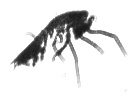
\includegraphics[width=0.4\textwidth]{kaggle_amphipod}
  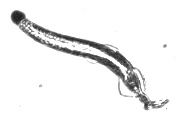
\includegraphics[width=0.4\textwidth]{kaggle_chaetognath}
  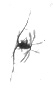
\includegraphics[width=0.2\textwidth]{kaggle_copepod}
  \end{column}
\end{columns}



\source{Kaggle plankton classification challenge (https://www.kaggle.com)}

\end{frame}

%%%%%%%%%%%%%%%%%%%%%%%%%%%%%%%%%%%%
\begin{frame}{Using simulated data}

  \begin{itemize}[<+->]
  \item Using simulated data is convenient...
  \item ... but it has to be as similar as possible to the real data
  \item A transfer learning method with real data will probably be necessary
  \item Your test data, of course, should be real
  \end{itemize}

\end{frame}


%%%%%%%%%%%%%%%%%%%%%%%%%%%%%%%%%%%%%%%%%%%%%%%%%%%%%
\section{Architecture choice}

%%%%%%%%%%%%%%%%%%%%%%%%%%%%%%%%%%%%
\begin{frame}{Architecture choice}

  \begin{itemize}[<+->]
  \item Begin with a standard architecture
    \begin{itemize}
    \item Classification problem: VGG, GoogLeNet, ResNet...
    \item Semantic segmentation or image transformation problem: U-Net
    \item Instance segmentation: Mask R CNN
    \end{itemize}
  \item If you are dealing with a complex problem, start with pre-learned weights and use transfer learning to adapt them to your application
  \end{itemize}

  \pause

  It is interesting to note that the rate of publication of new architectures tends to decrease.

\end{frame}


%%%%%%%%%%%%%%%%%%%%%%%%%%%%%%%%%%%%%%%%%%%%%%%%%%%%%
\section{Training}

%%%%%%%%%%%%%%%%%%%%%%%%%%%%%%%%%%%%
\begin{frame}{Optimizing your model}

  \begin{itemize}
  \item Choose an optimizer
  \item Use regularization ($L_1$, $L_2$, dropout, noise layer ...)
  \item Add batch normalization if convergence is difficult

  \end{itemize}

\end{frame}


%%%%%%%%%%%%%%%%%%%%%%%%%%%%%%%%%%%%
\begin{frame}{Hyperparameters tuning}

  Your options are:

  \begin{itemize}
  \item Manual tuning: works well if the number of parameter is small and the experience of the developer/researcher high
  \item Automatic tuning (grid search, random search): computationally time-consuming
  \end{itemize}

\end{frame}

%%%%%%%%%%%%%%%%%%%%%%%%%%%%%%%%%%%%
\begin{frame}{Computing power}

  DL became feasible in practice thanks to the use of Graphical Processing Units (GPU). Beyond theoretical research on the subject, to work with DL you need specific hardware:
  \begin{itemize}
  \item CPUs: with many of them, and using libraries that allow parallelization, this could be a solution - in practice, it is seldom done.
  \item GPUs: this is the most common solution adopted for deep learning. In practice, you need many of them. Note that you can either buy them or rent them online.
  \item TPU: Tensor Processing Units are integrated circuits specifically developed by Google for deep learning.
  \end{itemize}

\end{frame}

%%%%%%%%%%%%%%%%%%%%%%%%%%%%%%%%%%%%
\begin{frame}{Computing power}

  \begin{alertblock}{}
    \begin{itemize}
    \item   DL research and development is extremely computationally time-consuming.
    \item   However, a simple CPU is enough in most cases for running a given, already optimized, model.
    \end{itemize}
  \end{alertblock}
\end{frame}





%%%%%%%%%%%%%%%%%%%%%%%%%%%%%%%%%%%%%%%%%%%%%%%%%%

%%%%%%%%%%%%%%%%%%%%%%%%%%%%%%%%%%%%%%%%%%%%%%%%%%
%% \section*{References}

%% %%%%%%%%%%%%%%%%%%%%%%%%%%%%%%%%%%%%%%%%%%%%%%%%%%

%% \frame[allowframebreaks]{

%%   \scriptsize

%%   \frametitle{References}

%%   %\bibliographystyle{amsalpha}
%%   %\bibliographystyle{apalike}

%%   \bibliography{edf.bib}

%%   \normalsize

%% }




\end{document}
